\documentclass{report}
\usepackage{graphicx}
\usepackage{pdfpages}
\usepackage{blindtext}
\usepackage{titlesec}
\usepackage{polski}
\usepackage{hyperref}
\usepackage{listings}
\usepackage{xcolor}

%Ustawienie kolorowania tekstu docker-compose
\lstdefinelanguage{yaml}{
  morekeywords={version, services, image, volumes, ports, environment, volumes},
  sensitive=true,
  morecomment=[l][\color{gray}]{\#},
  morestring=[b][\color{blue}]{"},
  morestring=[b][\color{blue}]{'}
}

%Ustawienie kolorowania tekstu dla Dockerfile
\lstdefinestyle{dockerfile}{
    language=sh,
    backgroundcolor=\color{white},  
    basicstyle=\ttfamily\footnotesize,
    keywordstyle=\color{blue},       
    commentstyle=\color{green},   
    stringstyle=\color{red},      
    morekeywords={FROM, RUN, COPY, WORKDIR, ENTRYPOINT, CMD},
    numbers=left,
    stepnumber=1,
    numberstyle=\tiny\color{gray},
    numbersep=5pt,
    tabsize=2,
    breaklines=true,
    showspaces=false,
    showstringspaces=false,
    showtabs=false,
    frame=single
}

\lstdefinestyle{nginx}{
    language=bash,
    keywordstyle=\color{blue}\bfseries,
    commentstyle=\color{green},
    stringstyle=\color{red},
    basicstyle=\ttfamily\footnotesize,
    numbers=left,
    numberstyle=\tiny\color{gray},
    frame=single,
    breaklines=true,
    showstringspaces=false,
    morekeywords={server, location, listen, root, index, try_files, fastcgi_pass, fastcgi_param, fastcgi_intercept_errors, deny}
}

%Ustawienie spisu treści
\titleformat{\chapter}[hang]{\Huge\bfseries}{\thechapter}{1em}{} 
\renewcommand*\contentsname{Spis treści}

%Ustawienie rozmiarów
\titlespacing{\section}{0pt}{12pt}{6pt}
\titlespacing{\subsection}{0pt}{6pt}{6pt}
\usepackage[left=2.5cm,right=2.5cm,top=2.5cm,bottom=2.5cm]{geometry}

%Początek dokumentu
\begin{document}

%Strona tytułowa
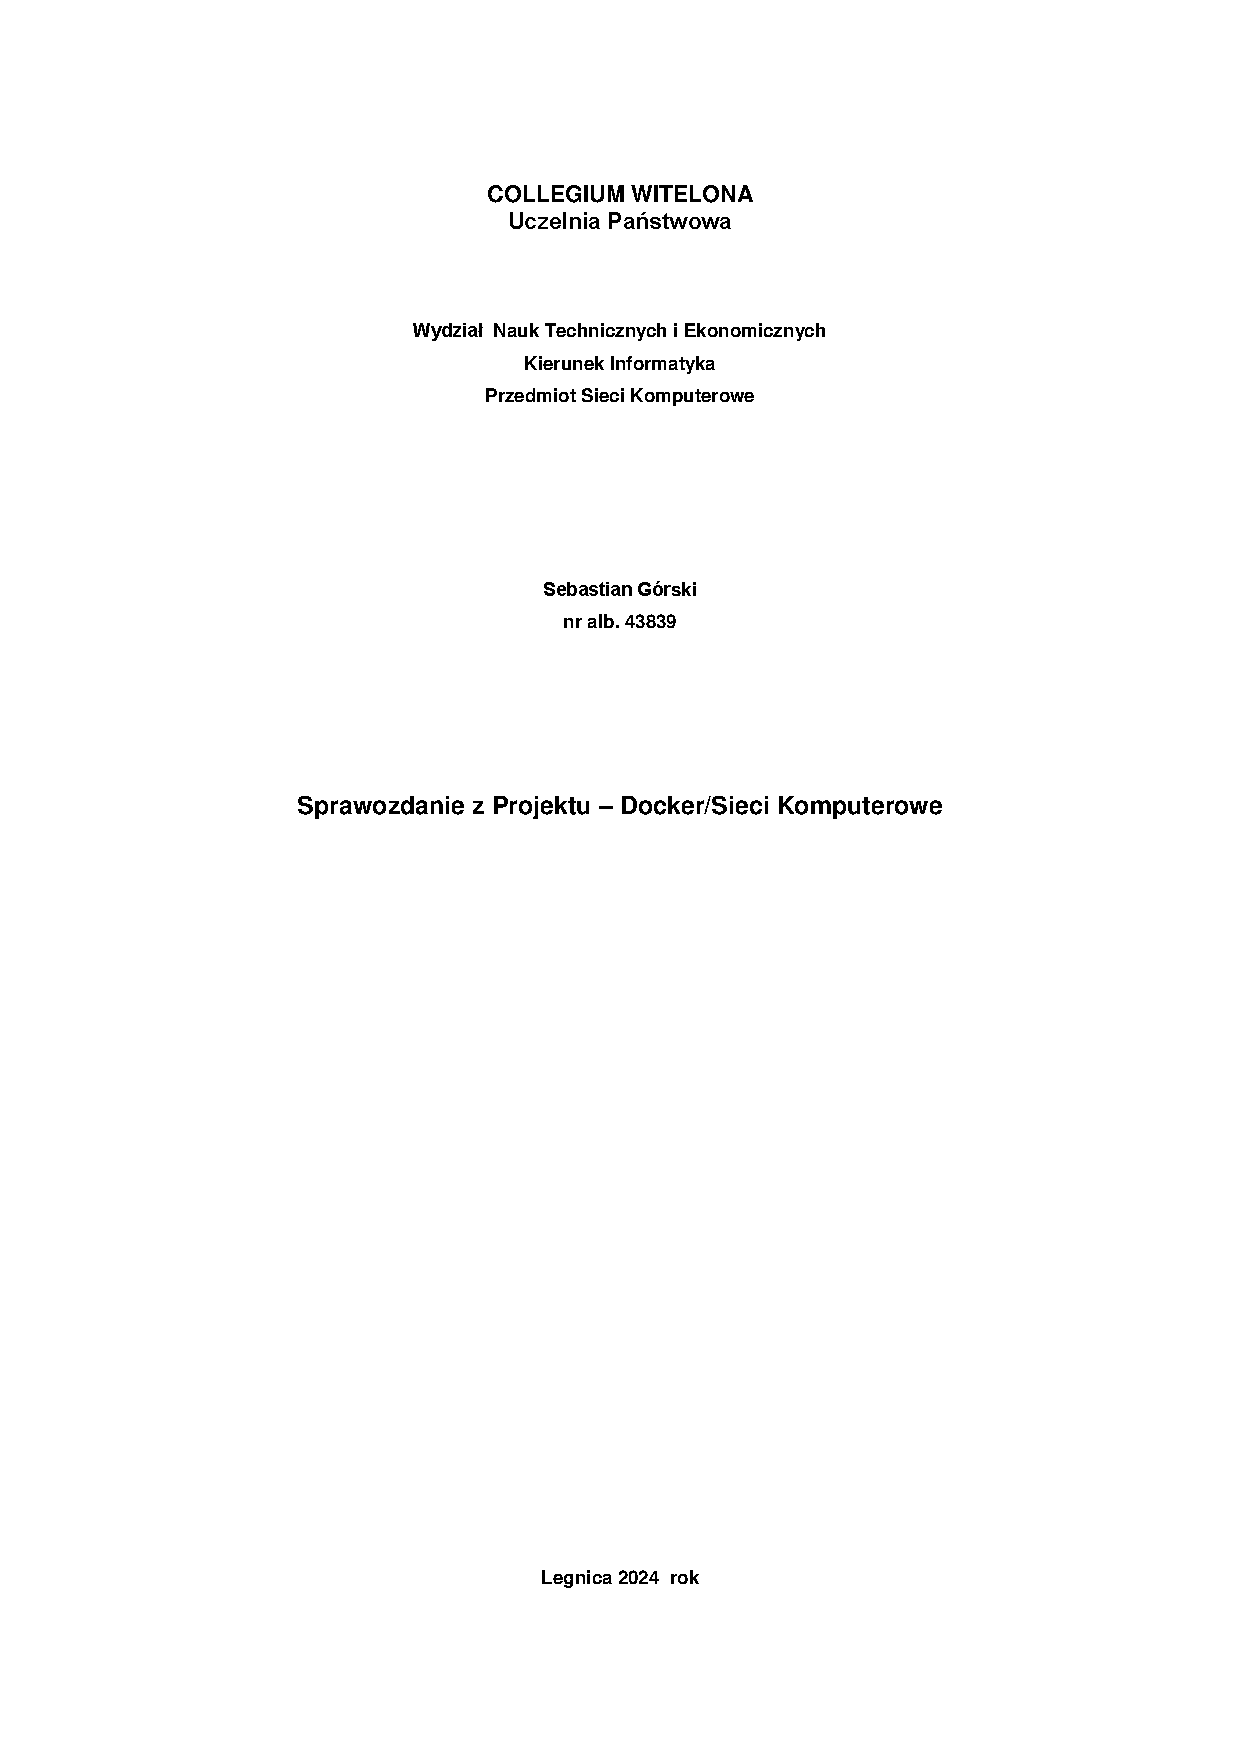
\includepdf[pages=-]{images/title-page.pdf}

%Spis treści
\tableofcontents
\newpage

%Rozdziały
\chapter{Wstęp}

\section{Opis projektu} 
Projekt miał na celu przygotowanie konfiguracji technologii Docker, która umożliwi łatwe uruchamianie aplikacji webowej „CN-Project”. Aby osiągnąć oczekiwany efekt, konieczne było utworzenie kontenerów zawierających niezbędne usługi, takie jak: serwer aplikacji PHP z frameworkiem Laravel, baza danych MySQL, serwer Nginx oraz system cache Redis. Dzięki użyciu Dockera możliwe będzie zapewnienie jednorodnego środowiska pracy dla wszystkich członków zespołu, bez potrzeby ręcznego instalowania i konfigurowania aplikacji oraz jej zależności na każdym komputerze.

\section{Podjęte kroki} 
Aby przygotować odpowiednie środowisko, zostały podjęte następujące kroki: 
\begin{enumerate} 
    \item Zainstalowanie programu Docker na stacji roboczej. 
    \item Utworzenie pliku \verb|docker-compose.yml| w folderze głównym projektu. 
    \item Utworzenie potrzebnych plików konfiguracyjnych. 
    \item Konfiguracja projektu. 
    \item Automatyzacja uruchomienia aplikacji. 
\end{enumerate}

\section{Cele projektu}
Główne cele wykonanego projektu to: 
\begin{enumerate} 
    \item Szybkie i spójne środowisko deweloperskie: Dzięki Dockerowi każdy deweloper w zespole może uruchomić projekt na swoim komputerze w identycznym środowisku, eliminując problemy związane z różnicami w konfiguracji lokalnych maszyn. 
    \item Automatyzacja instalacji i konfiguracji: Projekt automatyzuje proces instalacji wszystkich niezbędnych komponentów aplikacji, takich jak PHP, MySQL, Redis oraz Nginx, co pozwala na oszczędność czasu przy wdrażaniu nowego środowiska. 
    \item Skalowalność i łatwość rozwoju: Użycie kontenerów pozwala na łatwe dodawanie nowych usług, takich jak Node.js czy NPM, w przyszłości. 
    \item Izolacja usług: Każda z usług działa w osobnym kontenerze, co ułatwia zarządzanie nimi niezależnie. 
\end{enumerate}
\chapter{Instrukcja uruchomienia}

\section{Przed rozpoczęciem}
Przed uruchomieniem projektu należy upewnić się, że posiadane są wymagane składniki:

\begin{itemize}
    \item \textbf{Program Docker} - Jeżeli Docker nie jest zainstalowany na komputerze, należy go pobrać i zainstalować zgodnie z instrukcją na oficjalnej stronie: \href{https://docs.docker.com/desktop/}{https://docs.docker.com/desktop/}. 
    \item \textbf{Aplikacja CN-Project} - Należy upewnić się, że projekt znajduje się na używanej maszynie i nic nie blokuje dostępu do niego. Jeżeli projekt nie znajduje się na lokalnym sprzęcie, należy go pobrać przy użyciu programu Git i komendy: 
    \begin{quote} 
        \texttt{git clone https://github.com/KarolZygadlo/CN-Project.git} 
    \end{quote} 
\end{itemize}

\section{Uruchomienie projektu}
Aby uruchomić projekt „CN-Project” na swoim komputerze, należy wykonać następujące kroki:

\begin{enumerate} 
    \item Uruchomić program Docker Desktop na swoim systemie operacyjnym. 
    \item W konsoli systemu operacyjnego przejść do folderu, w którym znajduje się projekt (folder nazywa się \texttt{CN-Project}). 
    \item Projekt zostanie uruchomiony po wpisaniu i zatwierdzeniu poniższej komendy. Uruchomi ona kontenery w tle: 
    \begin{quote} 
        \texttt{docker compose up -d} 
    \end{quote} 
    \textit{Flagi:} 
    \begin{itemize} 
        \item \texttt{-d} - oznacza uruchomienie kontenerów w trybie odłączonym (w tle), co pozwala na dalsze korzystanie z terminala. 
    \end{itemize} Jeżeli chcemy widzieć logi kontenerów na bieżąco, należy użyć tej samej komendy, ale bez flagi \texttt{-d}: 
    \begin{quote} 
        \texttt{docker compose up}
    \end{quote} 
    \textit{Uwaga: Proces uruchamiania może potrwać kilka minut, szczególnie przy pierwszym uruchomieniu, ponieważ Docker pobiera wszystkie niezbędne obrazy i zależności.} 
    \item Po pobraniu i uruchomieniu projektu, aplikacja webowa będzie dostępna pod adresem \texttt{localhost}. Należy wpisać ten adres w przeglądarkę, aby wyświetlić stronę główną aplikacji. 
    \item Aby wyłączyć kontenery, należy wpisać w konsolę komendę: 
    \begin{quote} 
        \texttt{docker compose down} 
    \end{quote} Ta komenda zatrzyma wszystkie uruchomione kontenery. 
\end{enumerate}

\section{Wejście do kontenera}
W przypadku, gdy konieczne jest skorzystanie z narzędzi wewnątrz kontenera, najlepszym sposobem jest uruchomienie powłoki kontenera z poziomu maszyny lokalnej.

Poniższe kroki opisują sposób uruchomienia powłoki kontenera PHP.

\begin{enumerate} 
    \item Kontener musi być włączony. Można to sprawdzić przy pomocy komendy: 
    \begin{quote} 
        \texttt{docker ps} 
    \end{quote} Komenda ta pokazuje tylko aktualnie włączone kontenery.
    
    Poniżej przykład wyniku wywołania komendy \texttt{docker ps}:
    \begin{figure}[h]
        \centering
        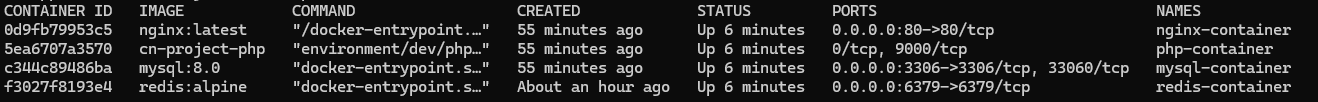
\includegraphics[width=\textwidth]{images/docker_ps.png}
    \end{figure}

    \textit{Ostatnia kolumna wskazuje nazwy kontenerów — nazwa kontenera będzie używana do odwoływania się do niego.}

    \item Korzystając z nazwy kontenera (np. \texttt{php-container}), można uruchomić powłokę kontenera PHP przy użyciu komendy:
    \begin{quote}
        \texttt{docker exec -it php-container sh}
    \end{quote}
    
    \textit{Elementy komendy:}
    \begin{itemize}
        \item \verb|docker exec -flagi [nazwa kontenera] [polecenia]| - wykonuje wybrane polecenie w wybranym konenerze. 
        \item \verb|-it| - Flaga \verb|-i| oznacza „interaktywny” tryb, co pozwala na komunikację z kontenerem, a \verb|-t| tworzy terminal, który umożliwia korzystanie z powłoki w trybie tekstowym.
        \item \verb|sh| - uruchamia powłokę systemu operacyjnego w kontenerze. Można używać innych powłok, takich jak \verb|bash|, jeżeli są dostępne w kontenerze.
    \end{itemize}
    
    Po zatwierdzeniu komendy użytkownik znajduje się wewnątrz kontenera i ma dostęp do wszystkich plików i programów, które się w nim znajdują.
\end{enumerate}
\chapter{Konfiguracja kontenerów}
Plik \verb|docker-compose.yml| to plik główny, wywoływany jako pierwszy przy użyciu technologii docker compose. Tutaj konfigurowane są wszystkie kontenery, sieci i wolumeny.
Plik jest podzielony na 3 części:
\begin{itemize}
    \item \verb|services| - tutaj znajduje się szczegółowa konfiguracja wszystkich konterów, które zostają uruchomione poprzez docker compose. Konfiguracje opisane są w tak zwanych usługach (\verb|service|). Sczegółowa analiza poszczególnych usług zostanie opisana w tym rozdziale.
    \item \verb|volumes| - w tym miejscu znajduje się wolumen o nazwie \textit{db-data}. Został utworzony, żeby dane były przechowywane w sposób trwały. Wolumen ten został wykorzystany w kontenerze bazy danych.
    \item \verb|networks| - w tej sekcji tworzona jest sieć dockera, w której będą działały wszystkie kontenery z sekcji \verb|services|. Jest to niezbędne do zapewnienia odpowiedniej łączności kontenerów między sobą. Sieć w tym projekcie nosi nazwę \textit{cn-network} i jest skonfigurowany do używania sterownika \verb|bridge|
\end{itemize}

Plik docker-compose jest plikiem w formacie YAML, którego struktura opiera się na wcięciach, a dane zapisywane są w formacie \verb|klucz: wartość|

\section{PHP}
PHP jest serwerowym językiem programowania kluczowym dla działania aplikacji, w tym projekcie skonfigurowanym z frameworkiem \verb|Laravel|, który usprawnia tworzenie aplikacji webowych. Użyto wersji PHP 8.2-fpm, zgodnej z Laravel 9 i nowszymi, zapewniającej wysoką wydajność dzięki FastCGI Process Manager (FPM).

Kontener PHP wzbogacono o dodatkowe zależności, takie jak Composer, zarządzający pakietami, oraz Redis, używany jako pamięć podręczna. Ten kontener obsługuje logikę aplikacji i komunikuje się z innymi usługami.
\subsection{docker-compose.yml}
Plik \verb|docker-compose.yml| definiuje konfigurację kontenera PHP.

\newpage
\begin{lstlisting}[language=yaml, caption={Konfiguracja kontenera php w pliku docker-compose.yml}, label={lst:docker_compose_php}, numbers=left, frame=single]
    php:
        build:
            context: .
            dockerfile: /environment/dev/php/Dockerfile
        container_name: php-container
        working_dir: /var/www
        volumes:
            - ./:/var/www
        expose:
            - "9000:9000"
        networks:
            - cn-network
        depends_on:
            - mysql
            - redis
\end{lstlisting}

W listingu \ref{lst:docker_compose_php} pokazana jest część pliku \verb|docker-compose| odpowiedzialna za utworzenie kontenera PHP. Można zauważyć, że sekcja ta dzieli się na kilka części.
\begin{itemize}
    \item \verb|build| - komenda używana do tworzenia obrazu kontenera na podstawie plików źródłowych.
    \begin{itemize}
        \item \verb|context| - miejsce wywołania pliku (\textit{. - aktualna ścieżka}).
        \item \verb|dockerfile| - lokalizacja pliku Dockerfile. W pliku Dockerfile został utworzony niestandardowy obraz na podstawie istniejącego już obrazu.
    \end{itemize}
    \item \verb|container_name| - nazwa kontenera - pole nieobowiązkowe, system sam może nadać nazwę, ale tutaj użytkownik posiada większą kontrolę.
    \item \verb|working_dir| - określa katalog roboczy, w którym kontener rozpocznie pracę.
    \item \verb|volumes| - określa jakie katalogi i pliki zostaną zamontowane do kontera. Wszystkie pliki źródłowe aplikacji zostają przeniesione do katalogu /var/www w kontenerze PHP.
    \item \verb|expose| - określa porty, które kontener udostępnia innym kontenerom wewnątrz sieci (w tym przypadku inne kontenry będą mogły odnaleźć PHP na porcie 9000 w sieci cn-network).
    \item \verb|networks| - sieci, w których kontener będzie pracował (w przypadku tego projektu wszystkie kontenery będą pracowały w jednej sieci, żeby miały do siebie swobodny dostęp).
    \item \verb|depends_on| - komenda, w której można ustawić "priorytety" kontenerów. W tym przypadku kontener PHP zależy od kontenerów: \verb|mysql| i \verb|redis|, co oznacza, że PHP nie zostanie uruchomiony, dopóki wymienione kontenery nie zostaną uruchomione.
\end{itemize}

\subsection{Dockerfile}
Plik Dockerfile pozwala na utworzenie niestandardowego obrazu na podstawie obrazu pobranego z \verb|Docker Hub|. Do tego pliku odwołała się usługa php w sekcji \verb|build|. W pliku tym ważne jest wskazanie z jakiego obrazu bazowego należy korzystać.

\newpage
\begin{lstlisting}[style=dockerfile, caption={Konfiguracja obrazu php w pliku Dockerilfe}, label={lst:dockerfile}]
FROM php:8.2-fpm

RUN apt-get update && apt-get install -y \
    git \
    unzip \
    zip \
    libpq-dev \
    libonig-dev \
    libcurl4-gnutls-dev \
    libxml2-dev \
    && docker-php-ext-install pdo pdo_mysql bcmath mbstring xml

RUN pecl install redis \
    && docker-php-ext-enable redis

COPY --from=composer:latest /usr/bin/composer /usr/bin/composer

WORKDIR /var/www

COPY .env.example .env
COPY . .

ENTRYPOINT ["environment/dev/php/entrypoint.sh"]
CMD ["php-fpm"]
\end{lstlisting}

W listingu \ref{lst:dockerfile} obrazem bazowym jest php w wersji 8.2-fpm. Wyznacza się go za pomocą komendy FROM.

W późniejszych etap pracuje się na wybranym obrazie, modyfikując go w dowolny sposób.

W tym pliku kolejno:
\begin{enumerate}
    \item Aktualizowane i instalowane są wymagane przez \verb|Composer| biblioteki.
    \item Instalowane jest rozszerzenie Redis, po czym zostaje aktywowany.
    \item Kopiowany jest obraz najnowszej wersji \verb|Composera| do tworzonego obrazu PHP.
    \item Ustawiany jest katalog roboczy, dzięki czemu kolejne operacje będą w nim wykonywane.
    \item Kopiowany jest plik .env.example do pliku .env (w pliku tym są wszystkie zmienne projektu)
    \item Kopiowana jest cała zawartość programu.
    \item Uruchamiany jest skrypt \verb|entrypoint.sh|
    \item Uruchamiany jest proces php-fpm, który będzie nasłuchwiał i obsługiwał żądania.
\end{enumerate}

\subsection{Skrypt Entrypoint}
W projekcie, w celu instalacji \verb|composera| i wstępnej inicjalizacji plików, uzyty został skrypt w języku \verb|bash|.

\newpage
\begin{lstlisting}[language=bash, caption=Skrypt entrypoint.sh, label={lst:entrypoint}, numbers=left, frame=single]
#!/bin/bash

if [ ! -f .env ]; then
    cp .env.example .env
fi

if [ ! -d "vendor" ]; then
    composer install --no-dev --no-interaction --optimize-autoloader
fi

php artisan key:generate --force
php artisan migrate --force

exec php-fpm
\end{lstlisting}

Skrypt z listingu \ref{lst:entrypoint} wykonuje kilke kilka poleceń konsolowych w obrazie tworzonym w listingu \ref{lst:dockerfile}. Na początku kopiowany jest plik ze zmiennymi, ponieważ \verb|Laravel| potrzebuje niektórych danych w nim zawarych. Następnie instalowany jest composer.
Po instalacji generowany jest unikalny klucz szyfrujący dla aplikacji Laravel, który zostaje zapisany w pliku \verb|.env|. Następnie baza zostaje zmigrowana. Od teraz kontener PHP jest skofigurowany do pracy z frameworkiem \verb|Laravel|.
\section{MySQL}
W projekcie został użyty obraz MySQL w wersji 8.0 jako silnik bazy danych. Zostało to podyktowane wysoką wydajnością, kompatybilnością z używanym środowiskiem oraz łatowścią korzystania i konfigurowania. Baza danych jest niezbędnym elementem każdej nowoczesnej aplikacji, w szczególności webowej.

\subsection{docker-compose.yml}
Cała konfiguracja serwera \verb|MySQL| opiera się na 11 wierszach zapisanych w pliku \verb|docker-copmpose|.

\begin{lstlisting}[language=yaml, caption={Konfiguracja kontenera MySQL w pliku docker-compose.yml}, label={lst:docker_compose_mysql}, numbers=left, frame=single]
    mysql:
        image: mysql:8.0
        container_name: mysql-container
        ports:
            - "3306:3306"
        environment:
            - MYSQL_DATABASE=${DB_DATABASE}
            - MYSQL_ROOT_PASSWORD=${DB_PASSWORD}
        volumes:
            - db-data:/var/lib/mysql
        networks:
            - cn-network
\end{lstlisting}

W tym przypadku, w przeciwieństwie do konfiguracji PHP nie używamy klucza \verb|build|, tylko \verb|image|. Określamy w nim bezpośrednio obraz, z którego będziemy korzystać. Nowym kluczem jest również klucz \verb|ports|. Jest to klucz porównywalny do \verb|expose|, z taką różnicą, że port ten jest widoczny zewnątrz dockera - możemy np. dostać się do niego przez przeglądarkę.
Dochodzi tutaj również klucz \verb|environment|, który zawiera listę zmiennych. W konfiguracji użyta została tylko nazwa bazy danych i hasło do konta użytkowanika root. Dane te pobierane są z pliku .env, z pól, kórych nazwa jest wpisana w klamrach.

\textit{W kluczu environment można wpisać również wartości wprost, wtedy nie będą pobierane z pliku .env, tylko bezpośrednio z tekstu, który został wpisany jako wartość klucza.}

Ważny jest również klucz \verb|volumes|, w którym tworzymy wolumen łączący \verb|db-data| z folderem mysql w kontenerze. Sposób tworzenia wolumenu jest ukazany w listingu \ref{lst:docker_compose_vlm}

\begin{lstlisting}[language=yaml, caption={Wolumen db-data w pliku docker-compose.yml}, label={lst:docker_compose_vlm}, numbers=left, frame=single]
volumes:
    db-data:
\end{lstlisting}
\section{Nginx}
Kolejnym kluczowym elementem aplikacji webowej jest serwer HTTP. Do obsługi ruchu HTTP użyty został serwer \verb|Nginx|, który został skonfigurowany do prekazywania żądań do aplikacji PHP. Użyta została wersja \verb|latest|, co oznacz najnowszą wersję z możliwych. Zabieg ten ma na celu ciągłe aktualizacje, które zwiększą bezpieczeństwo aplikacji. Mimo zmieniającej się wersji serwera \verb|Nginx|, nie powinno tworzyć to problemów. Serwer Nginx działa na porcie 80, czyli na nim aplikacja będzie uruchamiana.

\subsection{docker-compose.yml}
W tej sekcji konfiguracja jest prosta. Wszystkie klucze zostały omówione w poprzednich podrozdziałach dotyczących innych usług.

\begin{lstlisting}[language=yaml, caption={Konfiguracja kontenera Nginx w pliku docker-compose.yml}, label={lst:docker_compose_nginx}, numbers=left, frame=single]
    nginx:
        image: nginx:latest
        container_name: nginx-container
        ports:
            - "80:80"
        volumes:
            - ./environment/dev/nginx/nginx.conf:/etc/nginx/nginx.conf:ro
            - ./:/var/www
        networks:
            - cn-network
        depends_on:
            - php
\end{lstlisting}

\textit{Warto zwrócić uwagę na podpięcie pliku konfiguracyjnego do kontenera serwera HTTP. Znacznik :ro oznacza read-only (tylko do odczytu). Opis pliku znajduje się w rozdziale 3.3.2}

\subsection{nginx.conf}
Plik \verb|nginx.conf| definiuje w jaki sposób \verb|Nginx| ma obsługiwać przychodzące żądania. W przypadku tego proejktu jest podzielony na dwie sekcje - \verb|events| - listing \ref{lst:nginx_config_events} i \verb|http| - listing \ref{lst:nginx_config_http}.

\begin{lstlisting}[style=nginx, caption={Plik konfiguracyjny nginx.conf - sekcja events}, label={lst:nginx_config_events}]
events {
    worker_connections 1024;
}
\end{lstlisting}

W tym przypadku została określona liczba jednoczesnych połączeń na 1024.

\newpage
\begin{lstlisting}[style=nginx, caption={Plik konfiguracyjny nginx.conf - sekcja http}, label={lst:nginx_config_http}]
http {
    server {
        listen 80;
        server_name localhost;

        root /var/www/public;
        index index.php index.html;

        location / {
            try_files $uri $uri/ /index.php?$query_string;
        }

        location ~ \.php$ {
            include fastcgi_params;
            fastcgi_pass php-container:9000;
            fastcgi_param SCRIPT_FILENAME $document_root$fastcgi_script_name;
            fastcgi_intercept_errors on;
        }

        location ~ /\.ht {
            deny all;
        }
    }
}
\end{lstlisting}

Ta sekcja jest bardziej rozbudowana. Mówi między innymi o tym, że serwer \verb|Nginx| będzie nasłuchiwał na serwerze o nazwie localhost, na porcie 80. Katalog okreslony jako główny to /ver/www/public. Domyślnym plikiem indexowym jest plik \verb|index| z rozszerzeniem \verb|php| lub \verb|html|.

Następnie jest \verb|location /| - pole to określa w jaki sposób serwer ma obsłużyć żądanie HTTP wysłane na stronę. \verb|Nginx| spróbuje znaleźć plik lub katalog odpowiadający żądanej ścieżce. Jeśli ścieżka nie istnieje, pzekieruje żądanie do \verb|index.php| wraz z parametrami \verb|$query_string|.

Najdłuższa sekcja na liście to \verb|location ~ \.php$| - określa ona regułę obsługi wszystkich plików PHP. Skonfigurowane zostały tutaj niezbędne parametry do komunikacji z PHP. Najbardziej interesującym nas elementem jest \verb|fastcgi_pass| - ustawiamy tutaj, gdzie \verb|Nginx| ma szukać serwera PHP
\textit{Wpisana musi być nazwa kontenera, na którym jest uruchomiony PHP wraz z portem!}

Na koniec zablokowany jest dostęp do wszystkich plików, kórych nazwa zaczyna się od .ht (np. \verb|.htaccess|). Jest to istotne pod względem bezpieczeństwa aplikacji.
\section{Redis}
\verb|Redis| to system bazodanowy \verb|no-sql|, który działa w pamięci i przechowuje dane tymczasowe. Dzięki tej technologii zwiększa się wydajność aplikacji. Redis zostanie zintegrowany z kontenerem PHP i wspomoże dostęp do często używanych danych. Werjsa użyta w projekcie to \verb|Alpine| - najnowsza, lżejsza wersja technologii.

\subsection{docker-compose.yml}
\begin{lstlisting}[language=yaml, caption={Konfiguracja kontenera Redis w pliku docker-compose.yml}, label={lst:docker_compose_redis}, numbers=left, frame=single]
    redis:
        image: redis:alpine
        container_name: redis-container
        command: redis-server --appendonly yes
        ports:
            - "6379:6379"
        networks:
            - cn-network
\end{lstlisting}

W listingu \ref{lst:docker_compose_redis} widać konfigurację technologii \verb|Redis|. Nowością tutaj jest klucz \verb|command| z wartością \verb|redis-server --appendonly yes|. Klucz ten wywołuje komendę wpisaną w wartości poczas uruchomienia kontenera. Wartość \verb|redis-server| uruchamia serwer \verb|Redis|. Parametr \verb|--appendonly yes| włącza tryb zapisywania operacji do pliku.
\chapter{Podsumowanie}
W ramach projektu udało się stworzyć środowisko uruchomieniowe wykorzystując \verb|Docker compose| dla aplikacji webowej opartej na technologiach takich jak: \verb|PHP (Laravel), Nginx, MySQL i Redis|. Wykorzystana została do tego celu konfiguracja plikowa w plikach \verb|docker-compose.yml, Dockerfile| itd.

Konfiguracja ta pozwala na uruchomienie środowiska programistycznego na dowolnym komputerze, który posiada pliki źródłowe i program Docker.

Początkowo pojawiły się problemy związane z nieznajomością używanych technologii. Przez długi czas był problem z połączeniem bazy danych, przez co na stronie głównej pojawiał się błąd z rodziny 5xx. Rozwiązaniem okazało się zmienienie podejścia budowania niestandardowego obrazu PHP z Laravelem i momentu kopiowania pliku \verb|.env.example| do pliku \verb|.env|. Pomogło również zminimalizowanie konfiguracji do korzystania z użytkownika \verb|root| w konfiguracji \verb|MySQL|.

Z niewiadomych przczyn pojawił się również problem z wykorzystaniem PHP w standardowej wersji. W tym przypadku zmienienie obrazu na wersję \verb|FPM| oraz dodanie skryptu instalującego \verb|Composera|, zamiast instalowanie go w pliku \verb|Dockerfile| pomogło rozwiązać problem.

Środowisko mimo wszystko można jeszcze poprawić dodając nowe kontenery (np. \verb|PHPMyAdmin| lub \verb|Node.js|) oraz można popracować nad zwiększeniem wydajności.



\end{document}
